
\documentclass{article}
\usepackage{graphicx}
\usepackage{listings}

\graphicspath{ {../resources/} }

\begin{document}

\title{Blumengarten}
\author{Tassilo Tanneberger}

\maketitle

\section{Ideen der Algorithmen}
Ist eine sammlung an prinziplen Ideen die ich mir gemacht hatte befor ich angefangen hatt zu Implementieren.
\subsection{Bewertung von Farben}
 
\(w_i\) \dots  	Wichtung der Preferenz \newline
\(w_f\) \dots 	Finale Wichtung der Farbe \newline
\(N\) \dots    	Anzahl der Preferenzen mit dieser Farbe

\begin{equation}
w_f =  \sum \limits_{i=1}^N  (w_i^2 + 1)
\end{equation}

Diese Gleichung für die Wichtung hatt den Vorteil das durch das Quadrat die Wichtung des Nutzer mehr gewertet wird als wie oft er diese Farbe angab.

\subsection{Priotiry Places}

Jeder Platz auf dem Blumenbeet hatt eine gewisse anzahl an Nachbar Blumen n. Wobei n genau den Wert dieses Platzen repäsentiert. Dadurch das die anordung auch bis zu einem Gewissen grad Symetrisch ist kann  man nun anfangen die "wichtigen" Farben nun an wichtige Plätze packen. Somit ist mehr oder weniger eine feste reinfolge der Platzierungen gegeben wo zuerst die wichtigsten Farben (mit dem höchsten \(w_f\)) gesetzt werden.


\begin{figure}[h]
	\centering
	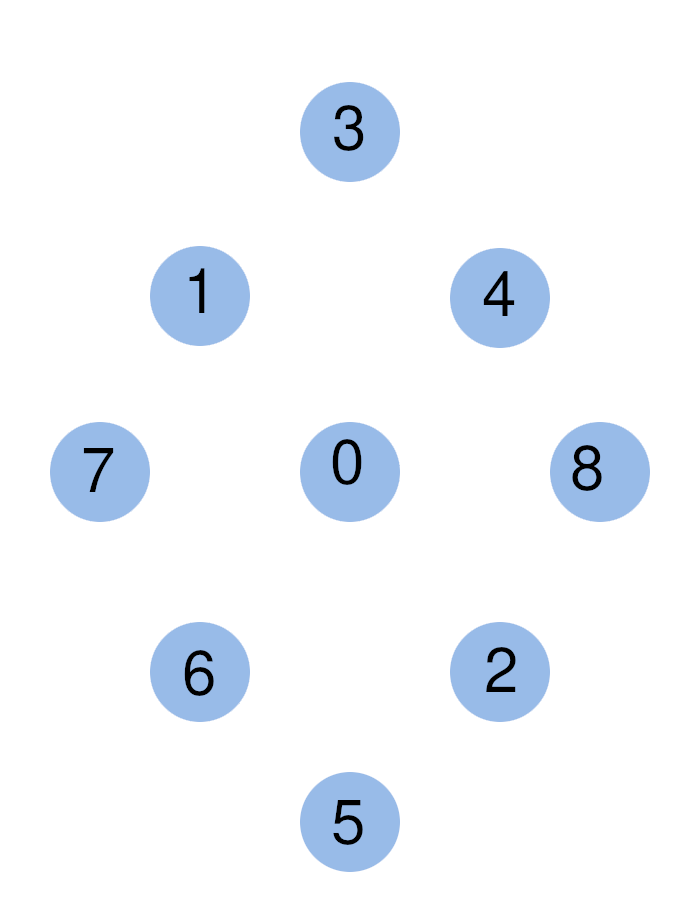
\includegraphics{priority_places}
	\caption{Reinfolge in der die Plätze vergeben werden}
\end{figure}


\newpage

Wobei hier zu beachten ist das 0, 1, 2 Immer mit den höchst gewichtesten Werten Platziert werden. Weil auch wenn alle 7 Farben genutzt werden sollen bleiben die \( 2 = 9 - 7\) für 1 und 2 übrig.

\section{Implementierung}

Alles wurde einfach aus einfachheits Gründen in Python3.7 Implementiert. Python als highlevel sprache ist einfach Ideal für solche klein Projeckte weil man sich z.B nicht um Memory Leaks, nervende Seq. Faults und ähnliches kümmern muss.

\newpage

\subsection{Sorted by Priority}

\subsubsection{ User Input }

Ich habe den Nutzer input etwas anders Designed indem ich zuerst die Prefernzen angeben lasse und danach frage ob er noch andere Farben möchte das macht mehr Sinn aus den einfachen Grund weil man somit Konflike vermeiden kann. Ein Beispiel der Nutzer sagt er möchte 2 Farben haben und sagt dann Rot-Blau-3 und Grün-Blau-2 und er hatt einen konflikt erzeugt weil er 3 Farben in den Prefernzen angiebt. anstelle nur von 2.


\subsubsection{Bewertung der Farben}

Implementierung der Bewertung. \newline

In Datei ./Blumengarten/Field.py
\begin{lstlisting}[language=Python]
    def __calcualate_value(self):

        self.colour_values: List[int] = [0] * 7

        # Element: 0 First Colour, 1 Second Colour, 2 Weight

        for element in self.user_input.preferences:

            self.colour_values[element[0]] += element[2] ** 2 + 1
            self.colour_values[element[1]] += element[2] ** 2 + 1	
	
\end{lstlisting}

Wobei preferences eine Liste mit Tupeln der Form (color1, color2, weight) ist.

\subsubsection{Generieren der anderen Farben}

Diese Methode erzeugt die zusätzlichen Farben zufällig. Zufällig einfach aus dem Grund um noch ein wenig variatät ins Spiel zu bringen.

\begin{lstlisting}[language=Python]
def generate_random_colors(self):
	self.additional_random: List[int] = []
	self.final_colors: List[int] = self.user_input.used_colors
	if self.user_input.colors_count > 0:
     	for x in range(self.user_input.colors_count):
         	ran: int = random.choice(self.user_input.open_colors)
         	del self.user_input.open_colors[self.user_input.open_colors.index(ran)]
         	self.additional_random.append(ran)
\end{lstlisting}


\subsubsection{Plazieren}

Als erstes werden die oben angesprochen freien besten Plätze statisch mit den besten Farben besetzt wie in der Reinfolge in Figure 1 beschrieben siehe Funktion placespare(). Wenn dieser Prozess abgeschlossen ist müssen wir alle Übrigen Farben noch unterbringen. Übrige Farben sind nun alle Zufälligen und nicht besten 2. Von diesen Farben wird es jeweils nur 1 geben. \break So nun wir wollen logischerweiße hier auch noch Punkte Sammeln bedeutet wir müssen uns für die Restlichen auch noch schauen wo wir sie am Klügsten hinplatzieren. Dafür gibt es folgene Einfache Schrittfolge:

\begin{enumerate}
\item Indices aller umliegender Plätzeheraus finden
\item Nach den Farben schaun die auf diesen Plätzen sich befinden
\item Dann wird die Farbe mit der Höchsten Synergie mit umliegenden Farben ermittelt
\item Farbe wird ins Feld geschrieben und aus den verfügbaren Farben heraus gestrichen
\end{enumerate}

\title Synergie Funktion

\begin{lstlisting}[language=Python]
    def query_highest_syn(self, color: list, already_used: list, possible_colors: list) -> int:
        ratings: List[int] = [0] * 7

        for x in possible_colors:
            if x in self.user_input.used_colors and x not in already_used:
                for c in color:
                    ratings[x] += Field.get(self.field.prepared, (c, x))

        if ratings == [0] * 7:
            i: int = random.choice(possible_colors)
        else:
            i: int = ratings.index(max(ratings))
        return i
\end{lstlisting}

Er Iteriert einfach durch die Verschiedenen Möglichkeiten machen weil es sehr übersichtlich viele Farben sind. Er Schaut ob die Farbe noch zur verfügung steht also in possiblecolors gelisted ist und nicht usedcolors ist. Dann schaut er sich die umliegenden Farben (color) an und fragt die wichtung zwichen diesen beiden Farben ab wenn es keine gibt ist der Wert einfach 0. Zum Schluss müssen wir dann noch schaun ob es überhaupt Synergien gab gab es keine Wird eine zufällige Farbe gewählt. Sonst der Wert der insgesamt die höchsten Synergien erreichte.



\end{document}